\documentclass{article}

\usepackage{graphicx}
\usepackage{tikz}
\usepackage{tikzsymbols}
\usetikzlibrary{calc,patterns,shapes.geometric}
\pagestyle{empty}
\usepackage[margin=0pt]{geometry}
\geometry{papersize={14in,12in}}

\def\centerarc[#1](#2)(#3:#4:#5){\draw[#1] ($(#2)+({#5*cos(#3)},{#5*sin(#3)})$) arc (#3:#4:#5);}

\begin{document}
	\begin{figure}
		\centering
		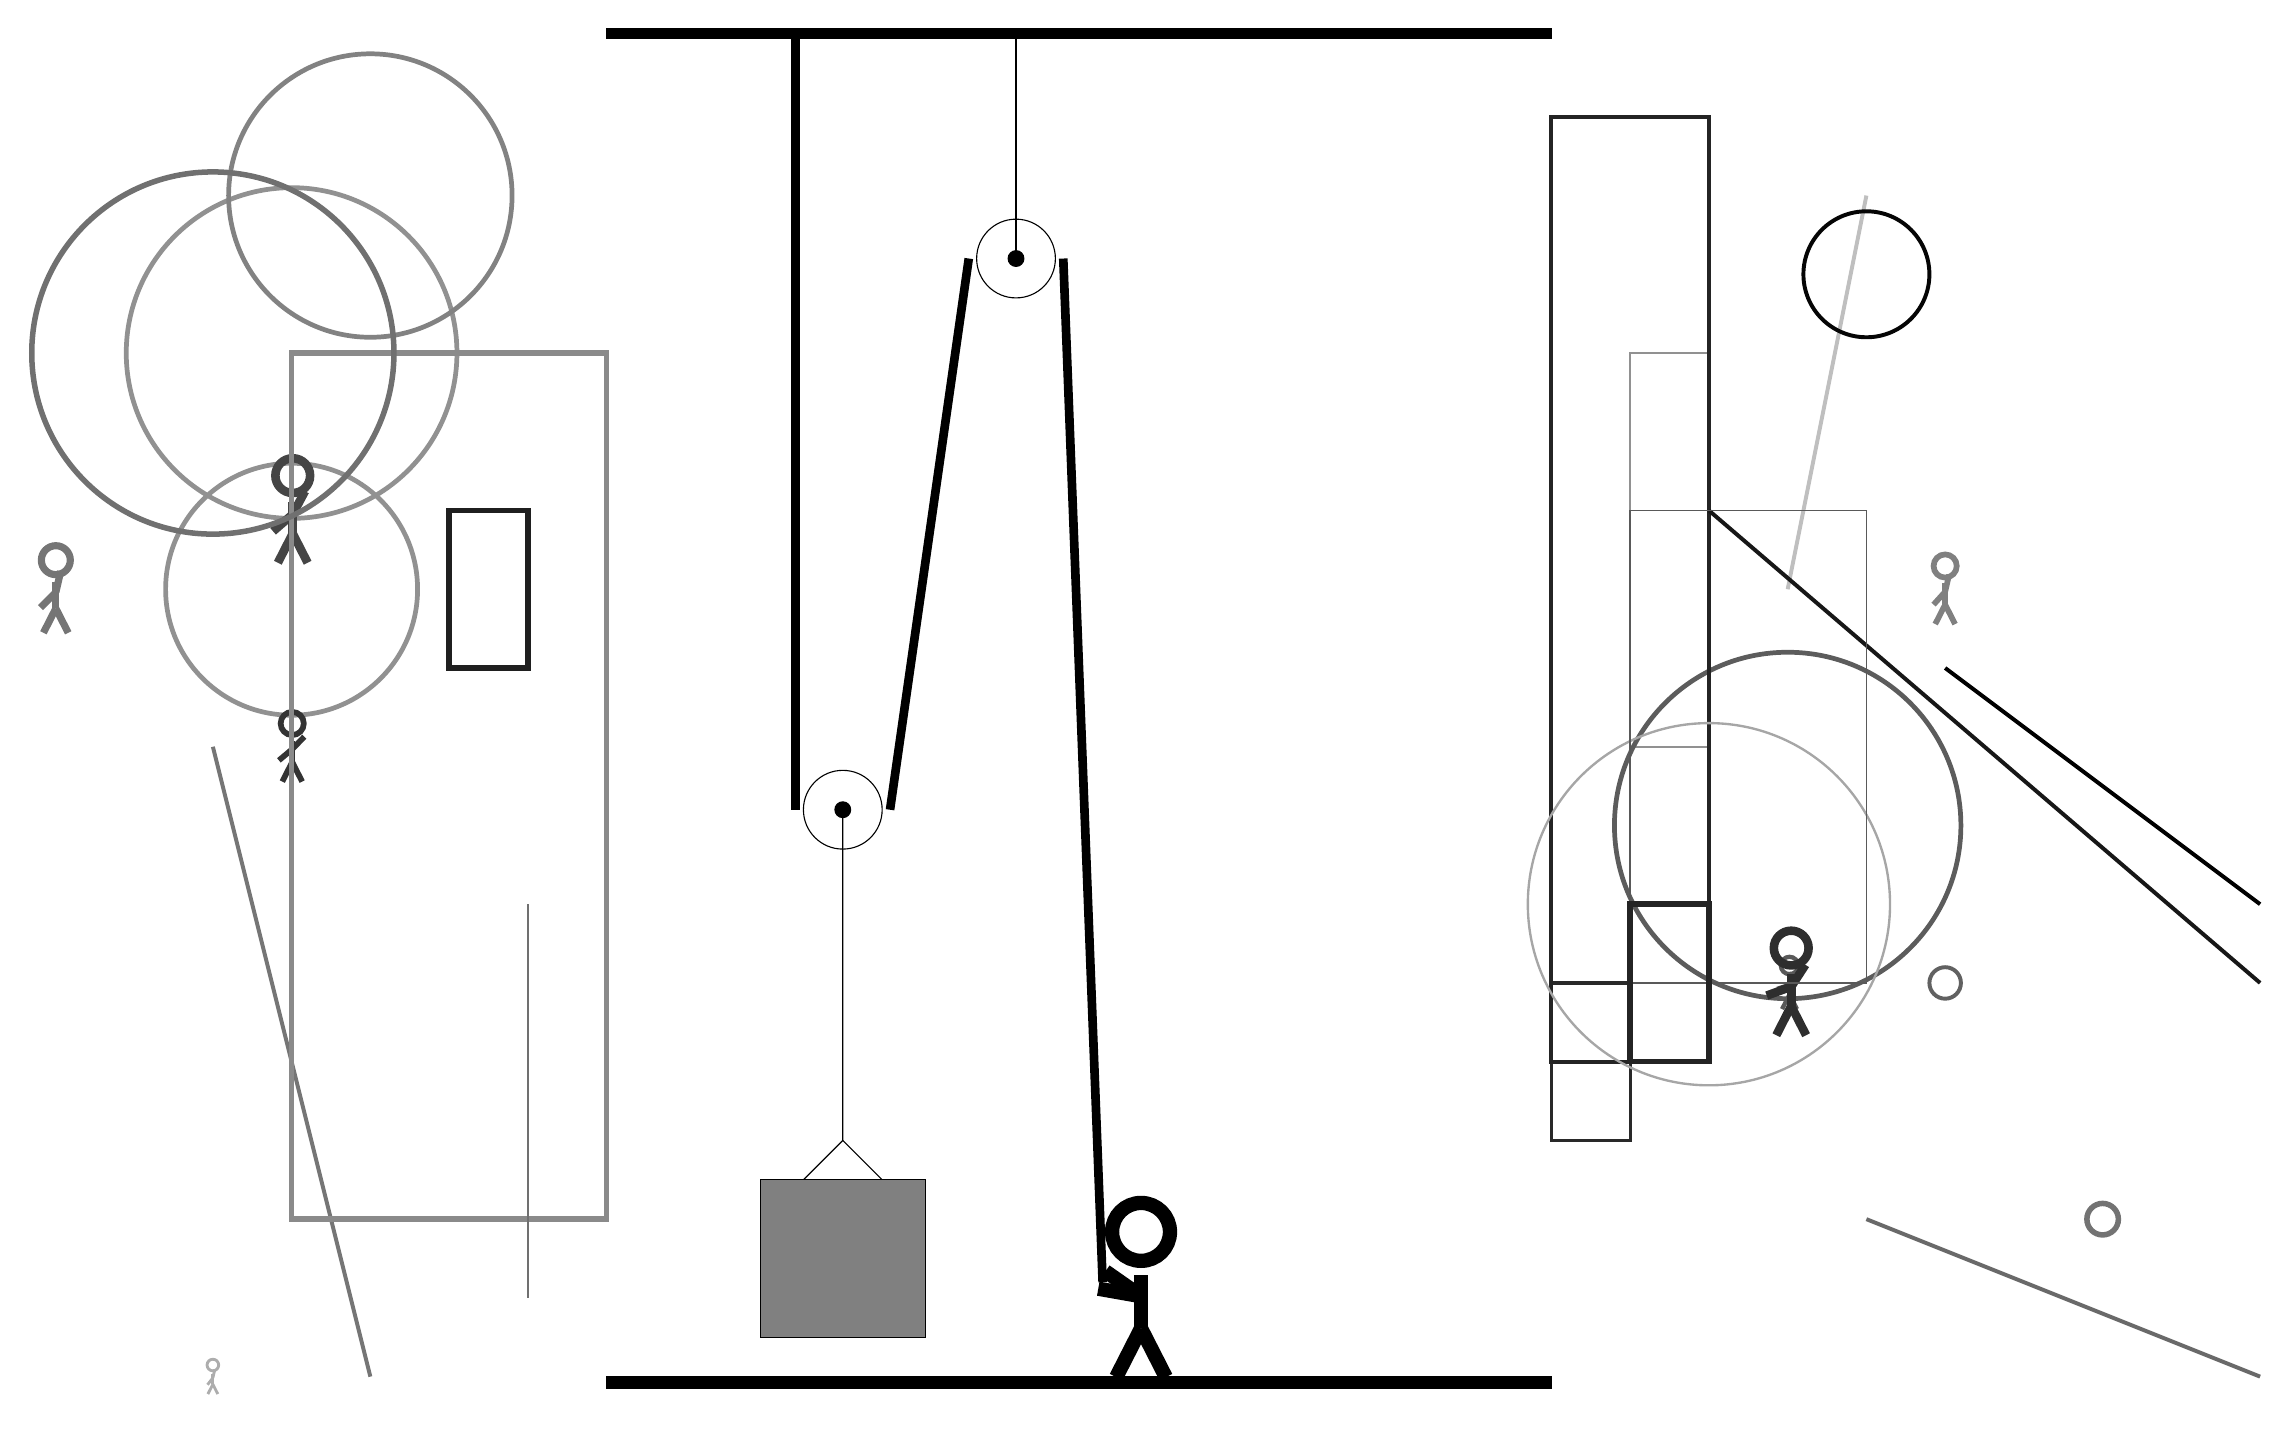
\begin{tikzpicture}
			%%%%% START %%%%%
			
			\draw[fill=black] (-2, 14) rectangle (10, 14.125);
			
			\draw (3.2, 11.2) circle (0.5);
			\draw[fill=black] (3.2, 11.2) circle (0.1);
			\draw[thick] (3.2, 11.2) -- (3.2, 14);
			
			\draw (1, 4.2) circle (0.5);
			\draw[fill=black] (1, 4.2) circle (0.1);
			
			\draw[line width=0.5mm, color=black!59](14, -1) -- (19, -3);
			
			\node[line width=0.4mm, color=black!32] at (-7, -3) {\Strichmaxerl[2][52][77]};
			\draw[line width=0.2mm, color=black!45] (12, 6) rectangle (12, 3);
			\draw[line width=0.5mm, color=black!100](15, 6) -- (19, 3);
			\draw [line width=0.6mm, color=black!43](-6, 10) circle (2.1);
			\draw[line width=0.3mm, color=black!43] (12, 10) rectangle (11, 5);
			
			\draw [line width=0.6mm, color=black!64](13, 4) circle (2.2);
			\draw[line width=0.4mm, color=black!84] (11, 0) rectangle (10, 2);
			\draw [line width=0.6mm, color=black!43](-6, 7) circle (1.6);
			
			\draw[line width=0.5mm, color=black!25](13, 7) -- (14, 12);
			\draw [line width=0.5mm, color=black!62](15, 2) circle (0.2);
			
			\draw[line width=0.5mm, color=black!86] (12, 13) rectangle (10, 1);
			\node[line width=0.7mm, color=black!65] at (13, 2) {\Strichmaxerl[3][18][79]};
			
			\node[line width=0.6mm, color=black!73] at (-6, 8) {\Strichmaxerl[6][41][62]};
			\draw [line width=0.5mm, color=black!98](14, 11) circle (0.8);
			\node[line width=0.7mm, color=black!82] at (13, 2) {\Strichmaxerl[6][20][57]};
			
			\draw[line width=0.5mm, color=black!91](12, 8) -- (19, 2);
			
			\draw[line width=0.5mm, color=black!54](-7, 5) -- (-5, -3);
			\node[line width=0.4mm, color=black!54] at (-9, 7) {\Strichmaxerl[5][45][77]};
			\draw [line width=0.3mm, color=black!35](12, 3) circle (2.3);
			\draw [line width=0.7mm, color=black!55](17, -1) circle (0.2);
			
			\node[line width=0.4mm, color=black!80] at (-6, 5) {\Strichmaxerl[4][40][46]};
			\draw[line width=0.7mm, color=black!46] (-2, -1) rectangle (-6, 10);
			\draw [line width=0.6mm, color=black!49](-5, 12) circle (1.8);
			\draw[line width=0.3mm, color=black!56] (-3, 3) rectangle (-3, -2);
			
			\draw [line width=0.7mm, color=black!56](-7, 10) circle (2.3);
			\node[line width=0.3mm, color=black!50] at (15, 7) {\Strichmaxerl[4][48][77]};
			\draw[line width=0.7mm, color=black!88] (-3, 6) rectangle (-4, 8);
			
			\draw[line width=0.2mm, color=black!65] (11, 8) rectangle (14, 2);
			\draw[line width=0.7mm, color=black!86] (11, 1) rectangle (12, 3);
			
			\draw (1, 4.2) -- (1, 0) -- (0.5, -0.5);
			\draw (1, 0) -- (1.5, -0.5);
			\draw[fill=black!50] (-0.05, -0.5) rectangle (2.05, -2.5);
			
			\draw[line width=1.1mm] (0.4, 14) -- (0.4, 4.2);
			\centerarc[line width=1.1mm](1, 4.2)(180:360:0.6);
			\draw[line width=1.1mm](1.6, 4.2) -- (2.6, 11.2);
			\centerarc[line width=1.1mm](3.2, 11.2)(0:180:0.6);
			\draw[line width=1.1mm](3.8, 11.2) -- (4.3, -1.8);
			
			\node at (4.7, -1.9) {\Strichmaxerl[10][-35][170]};
			
			\draw[fill=black] (-2, -3) rectangle (10, -3.15);
			
			%%%%% END %%%%%
		\end{tikzpicture}
	\end{figure}	
\end{document}